\section{Corpus-wide results}\label{sec:overview}

\subsection{Scale}
\nReviews{} reviews in \nOrgFolders{} taxon folders; \nAnn{} adjudicated existing annotations
(aspect resolved for \aspectMatched\% of rows); \nNew{} proposed new annotations; \nCoreFns{} core
functions; \nRefs{} reference entries; \nProposedTerms{} proposed GO terms; \nKnowledgeGaps{}
knowledge gaps. \todo{distribution of annotations per gene; taxon breakdown figure.}

\subsection{Overall action distribution}
\pctAccept\% \act{ACCEPT}, \pctKeepAsNonCore\% \act{KEEP\_AS\_NON\_CORE}, \pctModify\% \act{MODIFY},
\pctTooGeneral\% \act{TOO\_GENERAL}, \pctMarkAsOverAnnotated\% \act{MARK\_AS\_OVER\_ANNOTATED},
\pctRemove\% \act{REMOVE}, \pctUndecided\% \act{UNDECIDED}.
\emph{Protein binding} (\go{GO:0005515}{protein binding}) alone is \nPB{} rows (\pctPB\% of the
corpus) and is handled by policy (\S\ref{sec:dd-pb}); excluding it, \pctRejectedNoPB\% of
annotations are rejected (\act{REMOVE} or \act{MARK\_AS\_OVER\_ANNOTATED}) and \pctChangedNoPB\%
are changed in any way.

\note{Framing: a per-row error rate in the single digits is not the story. The story is that the
errors are \emph{concentrated} and \emph{systematic}: specific pipelines, codes and ontology
regions carry rejection rates several-fold above baseline, and because each is a mapping applied
proteome-wide, the absolute number of affected annotations in UniProt-GOA is large.
\todo{extrapolate: rejection rate per pipeline $\times$ pipeline size in current GOA.}}

\subsection{Errors by evidence class}
\begin{figure}[t]\centering
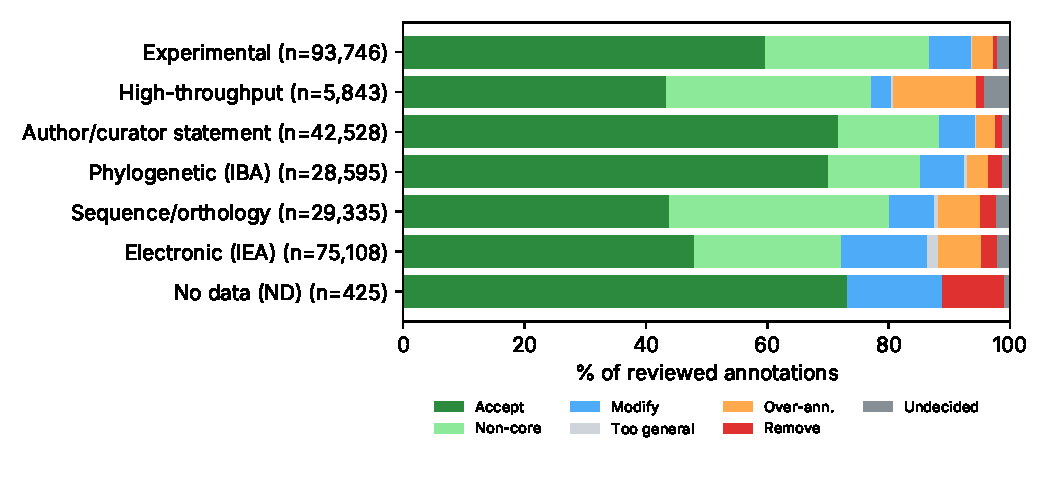
\includegraphics[width=\linewidth]{figures/action_by_evidence.pdf}
\caption{Review actions by evidence class (excluding protein binding).}
\label{fig:evidence}
\end{figure}

\begin{table}[t]\centering\scriptsize\setlength{\tabcolsep}{3pt}
\caption{Review actions (\% of rows) by evidence class, excluding protein binding.}
\label{tab:egroup}
% generated by scripts/compute_stats.py -- do not edit
\begin{tabular}{lrrrrrrrr}\toprule
Evidence class & $n$ & Accept & Non-core & Modify & Too general & Over-ann. & Remove & Undecided \\ \midrule
Experimental & 93,746 & 59.8 & 27.0 & 6.8 & 0.3 & 3.4 & 0.7 & 2.0 \\
High-throughput & 5,843 & 43.4 & 33.8 & 3.2 & 0.3 & 13.6 & 1.3 & 4.2 \\
Author/curator statement & 42,528 & 71.7 & 16.6 & 5.9 & 0.2 & 3.1 & 1.1 & 1.3 \\
Phylogenetic (IBA) & 28,595 & 70.1 & 15.1 & 7.1 & 0.6 & 3.5 & 2.3 & 1.2 \\
Sequence/orthology & 29,335 & 43.9 & 36.2 & 7.5 & 0.7 & 7.0 & 2.6 & 2.2 \\
Electronic (IEA) & 75,108 & 48.0 & 24.3 & 14.1 & 1.8 & 7.0 & 2.7 & 2.1 \\
No data (ND) & 425 & 73.2 & 0.0 & 15.8 & 0.0 & 0.0 & 10.1 & 0.9 \\
\bottomrule
\end{tabular}

\end{table}

Observations to develop:
\begin{itemize}[nosep]
  \item IBA is accepted at \accIBA\% (rejected \rejIBA\%), on a par with direct assays (IDA
        \accIDA\%) and well above other homology transfer (ISO \accISO\%, rejected \rejISO\%;
        ISS \accISS\%). Phylogenetically curated propagation behaves like experimental evidence;
        pairwise orthology transfer does not.
  \item Expression-pattern evidence (IEP) is the weakest experimental code (accepted \accIEP\%,
        rejected \rejIEP\%): expression is read as participation.
  \item High-throughput direct assays (HDA) are rejected at \rejHDA\% \todo{check: localisation proteomics?}.
  \item IEA is modified at \modIEA\% (vs IDA \modIDA\%): electronic terms are often right in
        kind but wrong in grain.
  \item Mutant phenotypes (IMP, IGI) are accepted at only \accIMP\% / \accIGI\%, with most of the
        remainder non-core: necessity is not participation.
\end{itemize}

\subsection{Errors by IEA pipeline}
\begin{table}[t]\centering\scriptsize\setlength{\tabcolsep}{3pt}
\caption{Review actions by electronic pipeline (GO\_REF), excluding protein binding.}
\label{tab:iea}
% generated by scripts/compute_stats.py -- do not edit
\begin{tabular}{lrrrrrrrr}\toprule
IEA pipeline & $n$ & Accept & Non-core & Modify & Too general & Over-ann. & Remove & Undecided \\ \midrule
Ensembl Compara orthology & 17,048 & 27.7 & 46.0 & 5.7 & 0.5 & 12.0 & 2.6 & 5.6 \\
InterPro2GO & 15,679 & 41.1 & 13.3 & 30.0 & 4.0 & 7.2 & 3.6 & 0.8 \\
Combined automated (UniProt) & 15,152 & 74.2 & 11.6 & 9.4 & 0.9 & 2.4 & 0.8 & 0.6 \\
UniProt subcellular location2GO & 9,349 & 63.0 & 25.5 & 7.1 & 0.6 & 2.1 & 0.6 & 1.1 \\
ARBA & 8,736 & 39.0 & 28.9 & 15.8 & 3.3 & 9.2 & 2.1 & 1.6 \\
UniProt keyword2GO & 2,906 & 44.4 & 14.6 & 22.1 & 2.7 & 9.3 & 6.6 & 0.3 \\
TreeGrafter & 1,501 & 43.7 & 22.9 & 9.6 & 0.9 & 8.6 & 10.4 & 4.0 \\
UniRule & 1,366 & 36.6 & 20.2 & 27.0 & 3.1 & 8.2 & 4.1 & 0.8 \\
GO logical inference & 1,154 & 35.8 & 23.7 & 10.0 & 0.3 & 14.0 & 14.0 & 2.3 \\
Rhea2GO & 832 & 60.9 & 19.7 & 10.7 & 0.8 & 4.9 & 1.3 & 1.6 \\
UniPathway2GO & 803 & 70.5 & 14.7 & 7.5 & 2.4 & 3.2 & 1.5 & 0.2 \\
EC2GO & 560 & 72.1 & 5.4 & 10.2 & 0.0 & 3.4 & 5.5 & 3.4 \\
\bottomrule
\end{tabular}

\end{table}
\note{Points: InterPro2GO is the most \act{MODIFY}-heavy (domain implies kind, not specificity);
GO logical inference and TreeGrafter have the highest rejection rates; Ensembl Compara orthology
has the lowest acceptance (most rows non-core or over-annotated, mainly BP from model-organism
phenotypes); UniProt-curated combined/subcellular-location rows are among the most reliable.}

\subsection{Errors by aspect and taxon}
\begin{table}[t]\centering\scriptsize\setlength{\tabcolsep}{3pt}
\caption{Review actions by GO aspect, excluding protein binding.}
\label{tab:aspect}
% generated by scripts/compute_stats.py -- do not edit
\begin{tabular}{lrrrrrrrr}\toprule
Aspect & $n$ & Accept & Non-core & Modify & Too general & Over-ann. & Remove & Undecided \\ \midrule
MF & 65,931 & 63.1 & 13.7 & 14.2 & 1.2 & 4.0 & 2.3 & 1.5 \\
BP & 106,286 & 42.8 & 36.1 & 8.1 & 0.9 & 7.6 & 1.8 & 2.6 \\
CC & 102,403 & 69.2 & 19.4 & 5.6 & 0.4 & 2.7 & 1.2 & 1.5 \\
\bottomrule
\end{tabular}

\end{table}
\todo{Biological process is the weak aspect (lowest acceptance); explain. Taxon table in
supplement (Table~\ref{tab:organism}).}

\subsection{Beyond existing annotations}
\todo{NEW annotations (\nNew): by aspect/evidence; proposed terms (\nProposedTerms); knowledge gaps
(\nKnowledgeGaps); source defects reported upstream; NOT candidates.}

\subsection{How reliable are the agent's calls?}
\todo{Essential for this title. Options: (a) blinded expert adjudication of a stratified random
sample of $\sim$500 decisions (per action $\times$ evidence class), reporting precision of
\act{REMOVE}/\act{MARK\_AS\_OVER\_ANNOTATED}; (b) agreement with upstream: fraction of
reported removals since acted on by GO/UniProt/MODs (cf.\ RAR re-examination); (c) re-review
stability across models/runs; (d) PR-review correction rate from history records.}
